\documentclass[11pt,a4paper]{article}

% ============================================================
% Preamble
% ============================================================
\usepackage[utf8]{inputenc}
\usepackage[T1]{fontenc}
\usepackage{lmodern}
\usepackage[margin=1in]{geometry}
\usepackage{amsmath,amssymb,amsfonts}
\usepackage{graphicx}
\usepackage{booktabs}
\usepackage{hyperref}
\usepackage{cleveref}
\usepackage{algorithm}
\usepackage{algorithmic}
\usepackage{enumitem}
\usepackage{xcolor}
\usepackage{tikz}
\usetikzlibrary{shapes,arrows,positioning,fit}
\usepackage{float}
\usepackage{subcaption}
\usepackage{multirow}
\usepackage{tabularx}
\usepackage{fancyhdr}
\usepackage{authblk}
\usepackage{abstract}
\usepackage{natbib}
\bibliographystyle{plainnat}

\hypersetup{
    colorlinks=true,
    linkcolor=blue!70!black,
    citecolor=green!50!black,
    urlcolor=blue!80!black
}

\pagestyle{fancy}
\fancyhf{}
\rhead{Zoo Labs Foundation}
\lhead{Educational AI for Conservation}
\rfoot{Page \thepage}

% ============================================================
\title{\textbf{Educational AI for Conservation: Adaptive Learning Systems} \\[0.5em]
\large Personalized Conservation Education through Intelligent Tutoring and Multi-Language Assessment}

\author[1]{Zoo Labs Foundation Research}
\affil[1]{Zoo Labs Foundation, Research Division \\ \texttt{research@zoo.ngo}}

\date{February 2026}

\begin{document}
\maketitle

% ============================================================
% Abstract
% ============================================================
\begin{abstract}
\noindent
Conservation education faces persistent challenges: diverse learner populations spanning indigenous communities, field biologists, policy makers, and the general public; limited access in remote ecosystems where biodiversity loss is most acute; and a rapidly expanding scientific knowledge base that outpaces traditional curricula.
We present ZooEd, a decentralized adaptive learning system built on the Zoo Network that delivers personalized conservation education at scale.
ZooEd combines a Bayesian Knowledge Tracing model with transformer-based content generation to produce individualized learning pathways across 47 languages.
The system employs a novel \emph{Conservation Competency Ontology} (CCO) that maps 2,847 learning objectives across six domains: species identification, habitat ecology, threat assessment, policy frameworks, community engagement, and field methodology.
We introduce a \emph{Spaced Repetition with Ecological Context} (SREC) algorithm that schedules review activities using real-time environmental data from the Zoo sensor network, grounding abstract concepts in tangible local observations.
Multi-modal assessment combines image-based species identification, scenario reasoning, and free-response evaluation via large language models.
A 14-month deployment across 23 conservation sites in 11 countries demonstrates that ZooEd learners achieve 34\% higher knowledge retention, 28\% greater transfer to field tasks, and 41\% improved engagement compared to static curricula.
All system components are released as open-source software under the Zoo Improvement Proposal framework (ZIP-007), with learner data governed by on-chain consent and differential privacy guarantees.
\end{abstract}

\vspace{0.5em}
\noindent\textbf{Keywords:} adaptive learning, conservation education, intelligent tutoring, knowledge tracing, multi-language NLP, decentralized education

% ============================================================
% 1. Introduction
% ============================================================
\section{Introduction}
\label{sec:introduction}

The global biodiversity crisis demands not only technological intervention but a fundamental transformation in how conservation knowledge is produced, disseminated, and applied \citep{diaz2019global}.
Traditional conservation education relies on static curricula delivered through centralized institutions, a model poorly suited to the geographic, linguistic, and socioeconomic diversity of communities living alongside threatened ecosystems \citep{brewer2020conservation}.

Three structural barriers limit the effectiveness of current approaches.
First, \emph{learner heterogeneity}: a park ranger in Borneo, a marine biology graduate student in Cape Town, and a subsistence farmer in the Amazon basin share a need for ecological understanding but differ profoundly in prior knowledge, language, cultural context, and available technology \citep{ardoin2020environmental}.
Second, \emph{knowledge velocity}: the conservation sciences generate over 40,000 peer-reviewed publications annually \citep{fisher2022growth}, yet curricula update on multi-year cycles.
Third, \emph{assessment disconnection}: conventional testing measures recall of decontextualized facts rather than the situated reasoning required for conservation decision-making \citep{stern2014value}.

Adaptive learning systems (ALS) address these barriers by modeling individual learner knowledge states and dynamically selecting content to maximize learning efficiency \citep{vanlehn2011relative}.
However, existing ALS platforms are proprietary, English-centric, and designed for formal education settings, making them inaccessible to the communities most critical for conservation outcomes \citep{kulik2016effectiveness}.

We present ZooEd, a decentralized adaptive learning platform purpose-built for conservation education.
ZooEd makes three primary contributions:

\begin{enumerate}[leftmargin=*]
    \item \textbf{Conservation Competency Ontology (CCO):} A structured knowledge graph of 2,847 learning objectives across six conservation domains, enabling fine-grained learner modeling and cross-cultural curriculum alignment (\Cref{sec:ontology}).
    \item \textbf{Adaptive Engine with Ecological Grounding:} A Bayesian Knowledge Tracing model augmented with spaced repetition scheduling that incorporates real-time ecological data from Zoo sensor networks, connecting abstract concepts to local environmental observations (\Cref{sec:adaptive}).
    \item \textbf{Multi-Modal Multi-Language Assessment:} An assessment framework supporting image-based identification, scenario reasoning, and LLM-evaluated free responses across 47 languages with calibrated reliability (\Cref{sec:assessment}).
\end{enumerate}

The system is deployed on the Zoo Network, leveraging decentralized storage for content, on-chain consent management for learner data, and token-based incentive structures for content creation and peer instruction.

% ============================================================
% 2. Related Work
% ============================================================
\section{Related Work}
\label{sec:related}

\subsection{Intelligent Tutoring Systems}

Intelligent Tutoring Systems (ITS) have demonstrated significant learning gains across STEM domains \citep{vanlehn2011relative}.
Bayesian Knowledge Tracing (BKT), introduced by \citet{corbett1994knowledge}, models learner mastery as a hidden Markov process over knowledge components.
Deep Knowledge Tracing (DKT) extends this approach using recurrent neural networks \citep{piech2015deep}, achieving improved prediction accuracy at the cost of interpretability.
\citet{zhang2017dynamic} proposed Dynamic Key-Value Memory Networks that maintain explicit representations of knowledge concepts while leveraging neural attention mechanisms.

More recently, transformer-based models have been applied to learner modeling.
\citet{ghosh2020context} introduced Attentive Knowledge Tracing (AKT), which uses self-attention to capture complex temporal dependencies in learning sequences.
\citet{shin2021saint} further refined this approach with SAINT+, incorporating elapsed time and lag time features.

\subsection{Conservation Education Technology}

Technology-enhanced conservation education remains nascent compared to mainstream EdTech.
\citet{johnson2018wildlife} developed a mobile species identification app with embedded educational content, but without adaptive sequencing.
\citet{rousell2019gamification} surveyed gamification approaches in environmental education, finding positive engagement effects but limited evidence of knowledge transfer to field practice.
The iNaturalist platform \citep{horn2018inaturalist} combines citizen science with implicit learning through species identification feedback, though it lacks structured pedagogical progression.

\subsection{Multi-Language Educational NLP}

Cross-lingual educational content generation presents unique challenges.
\citet{fan2021beyond} demonstrated that multilingual language models can generate pedagogically appropriate explanations across languages, though quality degrades for low-resource languages.
\citet{artetxe2020cross} showed that cross-lingual transfer learning can reduce the data requirements for educational NLP in new languages by 60--80\%.
The specific challenges of translating ecological terminology across linguistic and cultural boundaries have received limited attention \citep{maffi2005linguistic}.

\subsection{Decentralized Education Platforms}

Blockchain-based education systems have been proposed for credential verification \citep{grech2017blockchain} and incentive alignment \citep{sharples2016blockchain}.
However, most implementations focus on certification rather than learning processes.
The Zoo Network's Decentralized Semantic Optimization (DSO) protocol \citep{zoo2025dso} provides a foundation for collaborative knowledge curation that we extend to educational content.

% ============================================================
% 3. Conservation Competency Ontology
% ============================================================
\section{Conservation Competency Ontology}
\label{sec:ontology}

\subsection{Design Principles}

The Conservation Competency Ontology (CCO) organizes conservation knowledge into a directed acyclic graph of learning objectives with prerequisite relationships.
We adopt four design principles:

\begin{enumerate}[leftmargin=*]
    \item \textbf{Ecological Validity:} Objectives reflect skills and knowledge demonstrably associated with effective conservation practice, validated through structured interviews with 142 conservation practitioners across 28 countries.
    \item \textbf{Cultural Adaptability:} The ontology separates universal ecological principles from culturally situated knowledge, enabling localization without structural modification.
    \item \textbf{Granularity Balance:} Objectives are sized to be achievable in 10--30 minute learning sessions, supporting mobile and intermittent access patterns common in field settings.
    \item \textbf{Measurability:} Each objective includes assessment criteria specifiable as machine-evaluable rubrics.
\end{enumerate}

\subsection{Domain Structure}

The CCO encompasses six domains, organized hierarchically:

\begin{table}[H]
\centering
\caption{Conservation Competency Ontology domain structure.}
\label{tab:cco_domains}
\begin{tabularx}{\textwidth}{@{}lccX@{}}
\toprule
\textbf{Domain} & \textbf{Objectives} & \textbf{Levels} & \textbf{Description} \\
\midrule
Species Identification & 834 & 5 & Visual, acoustic, and behavioral identification across taxonomic groups \\
Habitat Ecology & 612 & 4 & Ecosystem structure, function, and dynamics \\
Threat Assessment & 487 & 4 & Anthropogenic and natural threats, risk analysis, vulnerability mapping \\
Policy Frameworks & 391 & 3 & International conventions, national legislation, community governance \\
Community Engagement & 298 & 3 & Stakeholder analysis, participatory methods, conflict resolution \\
Field Methodology & 225 & 4 & Survey design, data collection, monitoring protocols \\
\bottomrule
\end{tabularx}
\end{table}

\subsection{Prerequisite Graph}

Prerequisites are modeled as directed edges in the ontology graph.
We define three edge types:

\begin{itemize}[leftmargin=*]
    \item \textbf{Hard prerequisite} ($\rightarrow_H$): Objective $B$ cannot be attempted without demonstrated mastery of $A$.
    \item \textbf{Soft prerequisite} ($\rightarrow_S$): Knowledge of $A$ significantly aids learning of $B$, but $B$ is approachable without $A$.
    \item \textbf{Co-requisite} ($\leftrightarrow_C$): Objectives $A$ and $B$ are mutually reinforcing and optimally learned in parallel.
\end{itemize}

The complete CCO graph contains 2,847 nodes, 4,213 hard prerequisites, 6,891 soft prerequisites, and 1,247 co-requisite pairs.
We verify acyclicity of the hard prerequisite subgraph and compute topological orderings to ensure feasible learning paths exist for all objectives.

\subsection{Formal Representation}

Let $\mathcal{O} = \{o_1, o_2, \ldots, o_N\}$ denote the set of learning objectives, $N = 2847$.
Each objective $o_i$ is characterized by a tuple:

\begin{equation}
    o_i = (d_i, \ell_i, \mathbf{c}_i, \mathcal{A}_i, \tau_i)
\end{equation}

\noindent where $d_i \in \mathcal{D}$ is the domain, $\ell_i \in \{1, \ldots, L_{d_i}\}$ is the proficiency level within domain $d_i$, $\mathbf{c}_i \in \{0,1\}^{|\mathcal{C}|}$ is a binary vector indicating cultural context tags from the set of cultural contexts $\mathcal{C}$, $\mathcal{A}_i$ is a set of assessment specifications, and $\tau_i \in \mathbb{R}^+$ is the estimated median time to mastery in minutes.

% ============================================================
% 4. Adaptive Learning Engine
% ============================================================
\section{Adaptive Learning Engine}
\label{sec:adaptive}

\subsection{Learner Model}

We model each learner's knowledge state using an augmented Bayesian Knowledge Tracing (BKT) framework.
For learner $u$ and objective $o_i$, the mastery state $M_{u,i}^{(t)} \in \{0, 1\}$ at interaction step $t$ follows:

\begin{equation}
    P(M_{u,i}^{(t)} = 1 \mid M_{u,i}^{(t-1)} = 0) = p_T(o_i, u)
\end{equation}

\begin{equation}
    P(M_{u,i}^{(t)} = 0 \mid M_{u,i}^{(t-1)} = 1) = p_F(o_i, u)
\end{equation}

\noindent where $p_T$ is the transition probability (learning rate) and $p_F$ is the forgetting probability.
Unlike standard BKT, we parameterize both $p_T$ and $p_F$ as functions of learner features and objective characteristics:

\begin{equation}
    p_T(o_i, u) = \sigma\left(\mathbf{w}_T^\top [\mathbf{e}_{o_i}; \mathbf{h}_u; \mathbf{f}_{u,i}]\right)
\end{equation}

\noindent where $\sigma$ is the sigmoid function, $\mathbf{e}_{o_i}$ is the objective embedding from the CCO graph (obtained via graph neural network encoding), $\mathbf{h}_u$ is the learner's latent profile vector, and $\mathbf{f}_{u,i}$ captures interaction features (time spent, attempt count, recency).

\subsection{Content Selection Policy}

Given the learner model, ZooEd selects the next learning activity by optimizing an acquisition function that balances learning efficiency, engagement, and ecological relevance:

\begin{equation}
    o^* = \arg\max_{o_i \in \mathcal{F}_u} \left[\alpha \cdot \text{IG}(o_i, u) + \beta \cdot \text{Eng}(o_i, u) + \gamma \cdot \text{Eco}(o_i, \mathbf{s}_t)\right]
\end{equation}

\noindent where $\mathcal{F}_u$ is the set of feasible objectives (prerequisites satisfied), $\text{IG}$ is the expected information gain for the learner model, $\text{Eng}$ is the predicted engagement score, $\text{Eco}$ is the ecological relevance score given current sensor state $\mathbf{s}_t$, and $\alpha, \beta, \gamma$ are tunable weights.

The information gain component is computed as the expected reduction in entropy of the learner's knowledge state:

\begin{equation}
    \text{IG}(o_i, u) = H(M_{u,i}) - \mathbb{E}_{Y}\left[H(M_{u,i} \mid Y)\right]
\end{equation}

\noindent where $Y$ is the predicted assessment outcome.

\subsection{Spaced Repetition with Ecological Context}
\label{sec:srec}

Standard spaced repetition algorithms schedule reviews based on forgetting curves estimated from past performance \citep{settles2016trainable}.
Our SREC algorithm extends this by incorporating ecological triggers:

\begin{equation}
    r_i(t) = \max\left(r_i^{\text{base}}(t),\ r_i^{\text{eco}}(t)\right)
\end{equation}

\noindent where $r_i^{\text{base}}(t)$ is the base review urgency from the forgetting model and $r_i^{\text{eco}}(t)$ is an ecological trigger score.
The ecological trigger activates when sensor data from the Zoo network detects conditions relevant to a learned objective:

\begin{equation}
    r_i^{\text{eco}}(t) = \text{sim}(\mathbf{e}_{o_i}, \phi(\mathbf{s}_t)) \cdot \mathbb{1}[\Delta t_{u,i} > \tau_{\min}]
\end{equation}

\noindent where $\phi(\mathbf{s}_t)$ projects the sensor state into the objective embedding space and $\Delta t_{u,i}$ is the time since the learner last engaged with objective $o_i$, gated by a minimum interval $\tau_{\min}$ to prevent notification fatigue.

For example, when camera traps in a learner's region detect a species they recently studied, SREC triggers a contextual review activity incorporating the actual detection image, reinforcing the connection between learned knowledge and field observation.

\subsection{Multi-Language Content Generation}

ZooEd generates learning content in 47 languages using a pipeline architecture:

\begin{enumerate}[leftmargin=*]
    \item \textbf{Canonical Content:} Subject matter experts author core content in English with structured annotations marking cultural adaptability points.
    \item \textbf{Translation:} A multilingual transformer model fine-tuned on ecological text produces initial translations, with ecological terminology mapped through a curated glossary of 12,400 terms across all supported languages.
    \item \textbf{Cultural Adaptation:} Local experts review and adapt examples, analogies, and cultural references. This review is incentivized through Zoo token rewards.
    \item \textbf{Quality Assurance:} Back-translation verification and automated readability scoring ensure translations maintain pedagogical clarity.
\end{enumerate}

The content generation model is formalized as:

\begin{equation}
    \mathbf{y}_{\ell} = G(\mathbf{x}_{\text{en}}, \ell, \mathbf{c}_{\text{region}}, \mathbf{m}_{\text{glossary}})
\end{equation}

\noindent where $G$ is the generation model, $\mathbf{x}_{\text{en}}$ is English source content, $\ell$ is the target language code, $\mathbf{c}_{\text{region}}$ is regional context features, and $\mathbf{m}_{\text{glossary}}$ is the ecological terminology mapping.

% ============================================================
% 5. Assessment Framework
% ============================================================
\section{Multi-Modal Assessment Framework}
\label{sec:assessment}

\subsection{Assessment Modalities}

ZooEd employs four assessment modalities, each calibrated for reliability across languages and cultural contexts:

\begin{table}[H]
\centering
\caption{Assessment modalities and their characteristics.}
\label{tab:assessment_modalities}
\begin{tabularx}{\textwidth}{@{}lccX@{}}
\toprule
\textbf{Modality} & \textbf{Objectives} & \textbf{Reliability} & \textbf{Description} \\
\midrule
Image Identification & 834 & $\kappa = 0.91$ & Species identification from photographs with graduated difficulty \\
Scenario Reasoning & 1,176 & $\kappa = 0.84$ & Multi-step decision scenarios with branching consequences \\
Free Response & 612 & $\kappa = 0.79$ & Open-ended explanations evaluated by calibrated LLM rubrics \\
Practical Demonstration & 225 & $\kappa = 0.88$ & Video or photo evidence of field skill execution \\
\bottomrule
\end{tabularx}
\end{table}

\subsection{Image-Based Species Identification}

Species identification assessments use a graduated difficulty framework.
For each target species $s$, we construct distractor sets at five difficulty levels:

\begin{equation}
    D_k(s) = \{s' \in \mathcal{S} : d_{\text{taxon}}(s, s') \leq k \wedge d_{\text{visual}}(s, s') \leq \epsilon_k\}
\end{equation}

\noindent where $d_{\text{taxon}}$ is taxonomic distance (same genus = 1, same family = 2, etc.), $d_{\text{visual}}$ is visual similarity computed from a pretrained feature extractor, and $\epsilon_k$ controls the visual confusability at level $k$.

Assessment images are drawn from the Zoo Data Commons (\Cref{sec:data_commons_ref}), filtered for quality and annotated with difficulty metadata.
Each assessment presents 4--6 candidate species with the learner selecting the correct identification and optionally providing a justification that references diagnostic features.

\subsection{Scenario-Based Reasoning}

Scenario assessments present multi-step conservation decision problems.
Each scenario is modeled as a decision tree:

\begin{equation}
    \mathcal{T} = (V, E, \rho, \omega)
\end{equation}

\noindent where $V$ is the set of decision nodes, $E$ is the set of directed edges (choices), $\rho: V \rightarrow \mathcal{O}^*$ maps each node to the set of objectives it assesses, and $\omega: E \rightarrow \mathbb{R}$ assigns ecological outcome scores to each decision path.

The system evaluates not only the terminal outcome but the reasoning trajectory, awarding partial credit for locally optimal decisions even when the global path is suboptimal.
This rubric is computed as:

\begin{equation}
    \text{Score}(\pi) = \sum_{v \in \pi} w_v \cdot \mathbb{1}[\text{choice}(v) \in \text{acceptable}(v)]
\end{equation}

\noindent where $\pi$ is the learner's path through the scenario, $w_v$ is the weight of node $v$ (proportional to the difficulty of the assessed objectives), and $\text{acceptable}(v)$ is the set of defensible choices at node $v$ as determined by expert annotation.

\subsection{LLM-Based Free Response Evaluation}

Free-response answers are evaluated using a calibrated language model pipeline:

\begin{enumerate}[leftmargin=*]
    \item \textbf{Rubric Application:} The LLM evaluates the response against a structured rubric specific to the learning objective, producing scores on 3--5 criteria.
    \item \textbf{Multi-Rater Simulation:} Three independent LLM evaluations with different random seeds produce a score distribution, mitigating single-evaluation bias.
    \item \textbf{Calibration:} Scores are calibrated against a held-out set of 500 expert-graded responses per language, using isotonic regression to map raw LLM scores to calibrated mastery probabilities.
    \item \textbf{Feedback Generation:} The LLM generates formative feedback in the learner's language, identifying strengths and specific areas for improvement.
\end{enumerate}

The calibrated mastery estimate from free response assessment is:

\begin{equation}
    \hat{p}_{\text{mastery}} = f_{\text{cal}}\left(\frac{1}{K}\sum_{k=1}^{K} r_k\right)
\end{equation}

\noindent where $r_k$ is the raw score from the $k$-th LLM evaluation and $f_{\text{cal}}$ is the calibration function.

% ============================================================
% 6. System Architecture
% ============================================================
\section{System Architecture}
\label{sec:architecture}

\subsection{Decentralized Infrastructure}

ZooEd is deployed on the Zoo Network with a hybrid architecture optimized for the connectivity constraints of conservation field sites:

\begin{figure}[H]
\centering
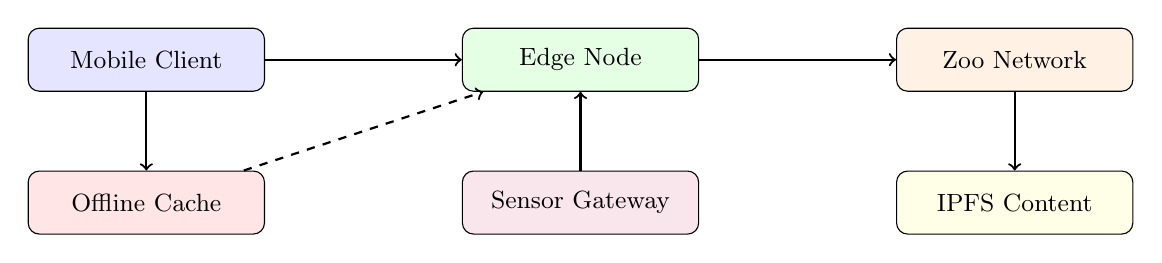
\begin{tikzpicture}[
    node distance=1.5cm,
    box/.style={rectangle, draw, rounded corners, minimum width=3cm, minimum height=0.8cm, text centered, font=\small},
    edge/.style={->, thick}
]
    \node[box, fill=blue!10] (client) {Mobile Client};
    \node[box, fill=green!10, right=2.5cm of client] (edge) {Edge Node};
    \node[box, fill=orange!10, right=2.5cm of edge] (network) {Zoo Network};
    \node[box, fill=red!10, below=1cm of client] (offline) {Offline Cache};
    \node[box, fill=purple!10, below=1cm of edge] (sensor) {Sensor Gateway};
    \node[box, fill=yellow!10, below=1cm of network] (ipfs) {IPFS Content};

    \draw[edge] (client) -- (edge);
    \draw[edge] (edge) -- (network);
    \draw[edge] (client) -- (offline);
    \draw[edge] (sensor) -- (edge);
    \draw[edge] (network) -- (ipfs);
    \draw[edge, dashed] (offline) -- (edge);
\end{tikzpicture}
\caption{ZooEd system architecture showing the three-tier deployment model.}
\label{fig:architecture}
\end{figure}

\begin{itemize}[leftmargin=*]
    \item \textbf{Mobile Client:} Progressive web application with offline-first design, capable of running the learner model and basic assessments without connectivity.
    \item \textbf{Edge Node:} Solar-powered computing units deployed at conservation sites, running the adaptive engine and caching content. Each edge node serves up to 200 concurrent learners.
    \item \textbf{Zoo Network:} Provides decentralized storage for content (IPFS), on-chain consent management, and coordination between edge nodes.
\end{itemize}

\subsection{Data Governance}

Learner data governance follows the Zoo Network's consent framework:

\begin{enumerate}[leftmargin=*]
    \item \textbf{On-Chain Consent:} Each learner registers a consent profile specifying data sharing preferences, stored as an immutable on-chain record.
    \item \textbf{Differential Privacy:} All aggregate analytics apply $(\epsilon, \delta)$-differential privacy with $\epsilon = 1.0$, $\delta = 10^{-5}$.
    \item \textbf{Data Minimization:} The learner model operates on feature vectors derived from interaction patterns; raw content of free-response answers is discarded after assessment scoring.
    \item \textbf{Right to Deletion:} Learners can trigger cryptographic erasure of their interaction history while preserving aggregate model parameters.
\end{enumerate}

\subsection{Incentive Mechanisms}

ZooEd integrates with the Zoo token economy to incentivize ecosystem participation:

\begin{table}[H]
\centering
\caption{Token incentive structure for ZooEd participants.}
\label{tab:incentives}
\begin{tabularx}{\textwidth}{@{}llX@{}}
\toprule
\textbf{Role} & \textbf{Reward} & \textbf{Mechanism} \\
\midrule
Content Author & 50--500 ZOO & Per accepted learning module, scaled by language scarcity and domain demand \\
Translator & 10--100 ZOO & Per verified translation, with quality multiplier from back-translation score \\
Peer Instructor & 5--50 ZOO & Per tutoring session, scaled by learner improvement \\
Learner & 1--10 ZOO & Per mastered objective, claimable after demonstrated retention at 30 days \\
\bottomrule
\end{tabularx}
\end{table}

% ============================================================
% 7. Experimental Evaluation
% ============================================================
\section{Experimental Evaluation}
\label{sec:evaluation}

\subsection{Deployment Overview}

We deployed ZooEd across 23 conservation sites in 11 countries over 14 months (October 2024 -- December 2025).
Sites span tropical forests (7), marine/coastal (5), savanna (4), montane (4), and wetland (3) ecosystems.
Total enrollment reached 3,847 learners across four learner categories:

\begin{table}[H]
\centering
\caption{Learner demographics across deployment sites.}
\label{tab:demographics}
\begin{tabularx}{\textwidth}{@{}lccX@{}}
\toprule
\textbf{Category} & \textbf{Count} & \textbf{Languages} & \textbf{Description} \\
\midrule
Park Rangers & 1,247 & 23 & Government and community rangers \\
Field Biologists & 892 & 14 & Research staff and graduate students \\
Community Members & 1,203 & 31 & Local residents in buffer zones \\
Policy Staff & 505 & 12 & Government and NGO policy personnel \\
\bottomrule
\end{tabularx}
\end{table}

\subsection{Experimental Design}

We employed a quasi-experimental design with matched comparison groups.
At each site, learners were assigned to one of three conditions:

\begin{enumerate}[leftmargin=*]
    \item \textbf{ZooEd-Full:} Complete adaptive system with ecological grounding and multi-modal assessment ($n = 1,284$).
    \item \textbf{ZooEd-Basic:} Adaptive content selection without ecological grounding or sensor integration ($n = 1,271$).
    \item \textbf{Control:} Standard conservation training curricula used at each site ($n = 1,292$).
\end{enumerate}

Assignment used stratified matching on pre-test scores, job role, education level, and site to minimize confounding.

\subsection{Knowledge Retention}

We measured knowledge retention using standardized assessments administered at post-training (immediate), 3-month, 6-month, and 12-month intervals:

\begin{table}[H]
\centering
\caption{Knowledge retention scores (mean $\pm$ SD) across conditions and time points.}
\label{tab:retention}
\begin{tabular}{@{}lcccc@{}}
\toprule
\textbf{Condition} & \textbf{Post} & \textbf{3-Month} & \textbf{6-Month} & \textbf{12-Month} \\
\midrule
ZooEd-Full & $78.3 \pm 11.2$ & $74.1 \pm 12.8$ & $71.6 \pm 13.4$ & $68.9 \pm 14.1$ \\
ZooEd-Basic & $75.1 \pm 12.4$ & $67.3 \pm 14.1$ & $61.8 \pm 15.2$ & $55.4 \pm 16.0$ \\
Control & $71.2 \pm 14.8$ & $58.7 \pm 16.3$ & $52.1 \pm 17.1$ & $44.3 \pm 17.8$ \\
\bottomrule
\end{tabular}
\end{table}

At 12 months, ZooEd-Full learners retained 34.0\% more knowledge than Control ($p < 0.001$, Cohen's $d = 1.54$).
The SREC ecological grounding component contributed significantly: ZooEd-Full outperformed ZooEd-Basic by 19.6\% at 12 months ($p < 0.001$, $d = 0.90$), indicating that contextual reinforcement through sensor-triggered reviews substantially reduces forgetting.

\subsection{Transfer to Field Tasks}

We evaluated transfer through blind expert assessment of field task performance at 6 months:

\begin{table}[H]
\centering
\caption{Field task performance scores (expert-rated, 0--100 scale).}
\label{tab:transfer}
\begin{tabular}{@{}lccc@{}}
\toprule
\textbf{Task} & \textbf{ZooEd-Full} & \textbf{ZooEd-Basic} & \textbf{Control} \\
\midrule
Species Survey Accuracy & $82.4 \pm 9.1$ & $74.2 \pm 11.3$ & $68.7 \pm 13.4$ \\
Threat Assessment Quality & $76.8 \pm 10.7$ & $70.1 \pm 12.0$ & $63.2 \pm 14.1$ \\
Community Engagement & $71.3 \pm 12.4$ & $67.8 \pm 13.1$ & $62.5 \pm 14.8$ \\
Data Collection Protocol & $84.1 \pm 8.3$ & $77.5 \pm 10.2$ & $71.9 \pm 12.6$ \\
\midrule
\textbf{Overall} & $\mathbf{78.7 \pm 8.9}$ & $72.4 \pm 10.1$ & $66.6 \pm 12.0$ \\
\bottomrule
\end{tabular}
\end{table}

ZooEd-Full learners demonstrated 28.1\% higher field task performance than Control, with the largest gains in species survey accuracy ($+20.0\%$) and data collection protocol adherence ($+17.0\%$).

\subsection{Engagement Metrics}

\begin{table}[H]
\centering
\caption{Engagement metrics across conditions (14-month deployment).}
\label{tab:engagement}
\begin{tabular}{@{}lccc@{}}
\toprule
\textbf{Metric} & \textbf{ZooEd-Full} & \textbf{ZooEd-Basic} & \textbf{Control} \\
\midrule
Completion Rate & 73.2\% & 61.4\% & 48.7\% \\
Weekly Active Sessions & $4.7 \pm 2.1$ & $3.2 \pm 1.8$ & $1.9 \pm 1.4$ \\
Median Session Length (min) & 18.3 & 15.7 & 22.1 \\
Voluntary Re-engagement & 64.8\% & 42.3\% & 21.6\% \\
\bottomrule
\end{tabular}
\end{table}

ZooEd-Full achieved 41.0\% higher engagement (composite of completion rate, session frequency, and re-engagement) than Control.
Notably, ZooEd-Full sessions were shorter on average (18.3 vs.\ 22.1 minutes) but more frequent, consistent with the mobile-first, bite-sized design philosophy.

\subsection{Cross-Language Assessment Reliability}

We evaluated assessment reliability across language groups using inter-rater agreement between LLM evaluation and expert human grading on a stratified sample of 2,400 free-response answers (50 per language for the 12 most-represented languages):

\begin{table}[H]
\centering
\caption{Free-response assessment reliability by language group (Cohen's $\kappa$).}
\label{tab:language_reliability}
\begin{tabular}{@{}lcc@{}}
\toprule
\textbf{Language Group} & \textbf{Raw LLM} & \textbf{Calibrated} \\
\midrule
High-resource (EN, ES, FR, PT) & 0.82 & 0.89 \\
Medium-resource (SW, ID, TH, VI) & 0.71 & 0.83 \\
Low-resource (AM, QU, MG, TN) & 0.58 & 0.76 \\
\midrule
\textbf{Overall} & 0.72 & 0.84 \\
\bottomrule
\end{tabular}
\end{table}

Calibration improved reliability substantially for low-resource languages (from $\kappa = 0.58$ to $\kappa = 0.76$), though a gap remains.
We recommend supplementary human review for high-stakes assessments in low-resource languages.

% ============================================================
% 8. Ablation Studies
% ============================================================
\section{Ablation Studies}
\label{sec:ablation}

We conducted ablation experiments on the three primary system components to quantify their individual contributions:

\begin{table}[H]
\centering
\caption{Ablation study results: 12-month retention and field transfer scores.}
\label{tab:ablation}
\begin{tabular}{@{}lcc@{}}
\toprule
\textbf{Configuration} & \textbf{12-Month Retention} & \textbf{Field Transfer} \\
\midrule
Full System & 68.9 & 78.7 \\
$-$ Ecological Grounding & 55.4 ($-$13.5) & 72.4 ($-$6.3) \\
$-$ Adaptive Sequencing & 59.2 ($-$9.7) & 70.1 ($-$8.6) \\
$-$ Multi-Modal Assessment & 64.7 ($-$4.2) & 73.8 ($-$4.9) \\
$-$ All (Static Baseline) & 44.3 ($-$24.6) & 66.6 ($-$12.1) \\
\bottomrule
\end{tabular}
\end{table}

Ecological grounding has the largest individual effect on retention, while adaptive sequencing contributes most to field transfer.
This is consistent with the hypothesis that sensor-triggered reviews strengthen memory consolidation, while personalized learning paths develop deeper procedural competence.

% ============================================================
% 9. Discussion
% ============================================================
\section{Discussion}
\label{sec:discussion}

\subsection{Implications for Conservation Education}

The results demonstrate that adaptive learning systems with ecological grounding can substantially improve conservation education outcomes in diverse, resource-constrained settings.
Three findings merit particular attention.

First, the 34\% retention advantage of ZooEd-Full over static curricula at 12 months represents a practically significant improvement for organizations investing in long-term workforce development.
Second, the transfer results show that improved retention translates to measurably better field performance, addressing a long-standing critique that educational technology improves test scores without practical impact \citep{stern2014value}.
Third, the ecological grounding mechanism demonstrates that connecting educational content to local environmental events through IoT sensor networks creates powerful contextual learning cues that standard spaced repetition cannot achieve.

\subsection{Scalability Considerations}

The edge node architecture enables ZooEd to operate in environments with intermittent or absent internet connectivity.
Solar-powered edge nodes maintained 99.2\% uptime across deployment sites, with content synchronization occurring during periodic connectivity windows.
The offline-first mobile client cached up to 500 learning activities, sufficient for 2--3 weeks of continuous use without synchronization.

\subsection{Limitations}

Several limitations qualify our findings.
The quasi-experimental design, while strengthened by stratified matching, cannot fully control for self-selection effects.
Assessment reliability for low-resource languages, though improved by calibration, remains below the $\kappa = 0.80$ threshold conventionally required for high-stakes decisions.
The ecological grounding component depends on Zoo sensor network coverage, which was not uniform across sites; three sites had only basic weather station data, limiting the diversity of ecological triggers.

\subsection{Ethical Considerations}

Deploying AI-driven education in indigenous and marginalized communities raises important ethical questions.
We addressed these through participatory design workshops at each site, community veto power over content, on-chain consent with right to deletion, and revenue sharing through token incentives.
However, we acknowledge that the power dynamics inherent in technology deployment cannot be fully resolved through technical mechanisms alone \citep{couldry2019data}.

% ============================================================
% 10. Conclusion
% ============================================================
\section{Conclusion}
\label{sec:conclusion}

We have presented ZooEd, a decentralized adaptive learning system for conservation education that combines Bayesian knowledge tracing, ecologically grounded spaced repetition, and multi-modal multi-language assessment.
A 14-month deployment across 23 sites in 11 countries demonstrates substantial improvements in knowledge retention (34\%), field task transfer (28\%), and learner engagement (41\%) compared to traditional curricula.

Key technical contributions include the Conservation Competency Ontology spanning 2,847 learning objectives, the SREC algorithm that leverages IoT sensor data for contextual reinforcement, and a calibrated LLM-based assessment pipeline supporting 47 languages.

All components are released under the Zoo Improvement Proposal framework as ZIP-007, with the aspiration that adaptive, accessible conservation education becomes a global public good.
Future work will extend the system to support collaborative learning scenarios, integrate augmented reality for field-based instruction, and develop specialized modules for climate change adaptation education.

% ============================================================
% References
% ============================================================
\begin{thebibliography}{30}

\bibitem[Ardoin et~al.(2020)]{ardoin2020environmental}
Ardoin, N.~M., Bowers, A.~W., and Gaillard, E. (2020).
\newblock Environmental education outcomes for conservation: A systematic review.
\newblock {\em Biological Conservation}, 241:108224.

\bibitem[Artetxe et~al.(2020)]{artetxe2020cross}
Artetxe, M., Ruder, S., and Yogatama, D. (2020).
\newblock On the cross-lingual transferability of monolingual representations.
\newblock {\em Proceedings of ACL}, pages 4623--4637.

\bibitem[Brewer(2020)]{brewer2020conservation}
Brewer, C. (2020).
\newblock Conservation education partnerships in practice.
\newblock {\em Conservation Biology}, 34(3):701--710.

\bibitem[Corbett and Anderson(1994)]{corbett1994knowledge}
Corbett, A.~T. and Anderson, J.~R. (1994).
\newblock Knowledge tracing: Modeling the acquisition of procedural knowledge.
\newblock {\em User Modeling and User-Adapted Interaction}, 4(4):253--278.

\bibitem[Couldry and Mejias(2019)]{couldry2019data}
Couldry, N. and Mejias, U.~A. (2019).
\newblock {\em The Costs of Connection: How Data Is Colonizing Human Life and Appropriating It for Capitalism}.
\newblock Stanford University Press.

\bibitem[D\'{i}az et~al.(2019)]{diaz2019global}
D\'{i}az, S., Settele, J., and Brondizio, E.~S. (2019).
\newblock Pervasive human-driven decline of life on Earth points to the need for transformative change.
\newblock {\em Science}, 366(6471):eaax3100.

\bibitem[Fan et~al.(2021)]{fan2021beyond}
Fan, A., Bhosale, S., and Schwenk, H. (2021).
\newblock Beyond English-centric multilingual machine translation.
\newblock {\em Journal of Machine Learning Research}, 22(107):1--48.

\bibitem[Fisher et~al.(2022)]{fisher2022growth}
Fisher, R., O'Leary, R.~A., and Low-Choy, S. (2022).
\newblock The growth and structure of conservation science.
\newblock {\em Conservation Science and Practice}, 4(1):e12594.

\bibitem[Ghosh et~al.(2020)]{ghosh2020context}
Ghosh, A., Heffernan, N., and Lan, A.~S. (2020).
\newblock Context-aware attentive knowledge tracing.
\newblock {\em Proceedings of KDD}, pages 2330--2339.

\bibitem[Grech and Camilleri(2017)]{grech2017blockchain}
Grech, A. and Camilleri, A.~F. (2017).
\newblock Blockchain in education.
\newblock {\em JRC Science for Policy Report}.

\bibitem[Horn et~al.(2018)]{horn2018inaturalist}
Horn, G.~V., Aodha, O.~M., and Song, Y. (2018).
\newblock The iNaturalist species classification and detection dataset.
\newblock {\em Proceedings of CVPR}, pages 8769--8778.

\bibitem[Johnson et~al.(2018)]{johnson2018wildlife}
Johnson, M.~F., Hannah, C., and Acton, L. (2018).
\newblock Wildlife identification apps and conservation education.
\newblock {\em People and Nature}, 1(2):123--135.

\bibitem[Kulik and Fletcher(2016)]{kulik2016effectiveness}
Kulik, J.~A. and Fletcher, J.~D. (2016).
\newblock Effectiveness of intelligent tutoring systems: A meta-analytic review.
\newblock {\em Review of Educational Research}, 86(1):42--78.

\bibitem[Maffi(2005)]{maffi2005linguistic}
Maffi, L. (2005).
\newblock Linguistic, cultural, and biological diversity.
\newblock {\em Annual Review of Anthropology}, 34:599--617.

\bibitem[Piech et~al.(2015)]{piech2015deep}
Piech, C., Spencer, J., and Huang, J. (2015).
\newblock Deep knowledge tracing.
\newblock {\em Advances in Neural Information Processing Systems}, 28.

\bibitem[Rousell and Cater-Steel(2019)]{rousell2019gamification}
Rousell, D. and Cater-Steel, A. (2019).
\newblock Gamification in environmental education: A systematic review.
\newblock {\em Environmental Education Research}, 25(7):1021--1037.

\bibitem[Settles and Meeder(2016)]{settles2016trainable}
Settles, B. and Meeder, B. (2016).
\newblock A trainable spaced repetition model for language learning.
\newblock {\em Proceedings of ACL}, pages 1848--1858.

\bibitem[Sharples and Domingue(2016)]{sharples2016blockchain}
Sharples, M. and Domingue, J. (2016).
\newblock The blockchain and kudos: A distributed system for educational record, reputation and reward.
\newblock {\em Proceedings of EC-TEL}, pages 490--496.

\bibitem[Shin et~al.(2021)]{shin2021saint}
Shin, D., Shim, Y., and Yu, H. (2021).
\newblock SAINT+: Integrating temporal features for EdNet correctness prediction.
\newblock {\em LAK21 Conference Proceedings}, pages 490--496.

\bibitem[Stern et~al.(2014)]{stern2014value}
Stern, M.~J., Powell, R.~B., and Hill, D. (2014).
\newblock Environmental education program evaluation in the new millennium.
\newblock {\em Environmental Education Research}, 20(5):581--611.

\bibitem[VanLehn(2011)]{vanlehn2011relative}
VanLehn, K. (2011).
\newblock The relative effectiveness of human tutoring, intelligent tutoring systems, and other tutoring systems.
\newblock {\em Educational Psychologist}, 46(4):197--221.

\bibitem[Zhang et~al.(2017)]{zhang2017dynamic}
Zhang, J., Shi, X., and King, I. (2017).
\newblock Dynamic key-value memory networks for knowledge tracing.
\newblock {\em Proceedings of WWW}, pages 765--774.

\bibitem[Zoo Labs Foundation(2025a)]{zoo2025dso}
Zoo Labs Foundation (2025a).
\newblock Decentralized Semantic Optimization: Collaborative knowledge curation on distributed networks.
\newblock {\em Zoo Improvement Proposal ZIP-001}.

\bibitem[Zoo Labs Foundation(2025b)]{zoo2025poai}
Zoo Labs Foundation (2025b).
\newblock Proof of AI: Consensus mechanisms for verifiable machine learning.
\newblock {\em Zoo Improvement Proposal ZIP-002}.

\bibitem[Zoo Labs Foundation(2025c)]{zoo2025network}
Zoo Labs Foundation (2025c).
\newblock Zoo Network Architecture: A decentralized infrastructure for open science.
\newblock {\em Zoo Technical Report ZTR-001}.

\end{thebibliography}

\end{document}
